\documentclass[border=10pt]{standalone}
\usepackage[utf8]{inputenc}
\usepackage{tikz}
\usetikzlibrary{shapes,arrows,positioning,calc}

\tikzstyle{start} = [circle, fill=green!50, line width=2pt, minimum size=1.5cm]
\tikzstyle{end} = [circle, fill=red!30, line width=2pt, minimum size=1.5cm]
\tikzstyle{process} = [rectangle, rounded corners, draw=black, fill=blue!20, line width=1.5pt, minimum width=3.5cm, minimum height=0.9cm, text width=3.3cm, text centered, font=\small]
\tikzstyle{decision} = [diamond, draw=black, fill=yellow!30, line width=1.5pt, aspect=2, text width=2cm, text centered]
\tikzstyle{arrow} = [thick, ->, >=stealth]
\tikzstyle{loop} = [thick, dashed, ->, >=stealth, red]

\begin{document}

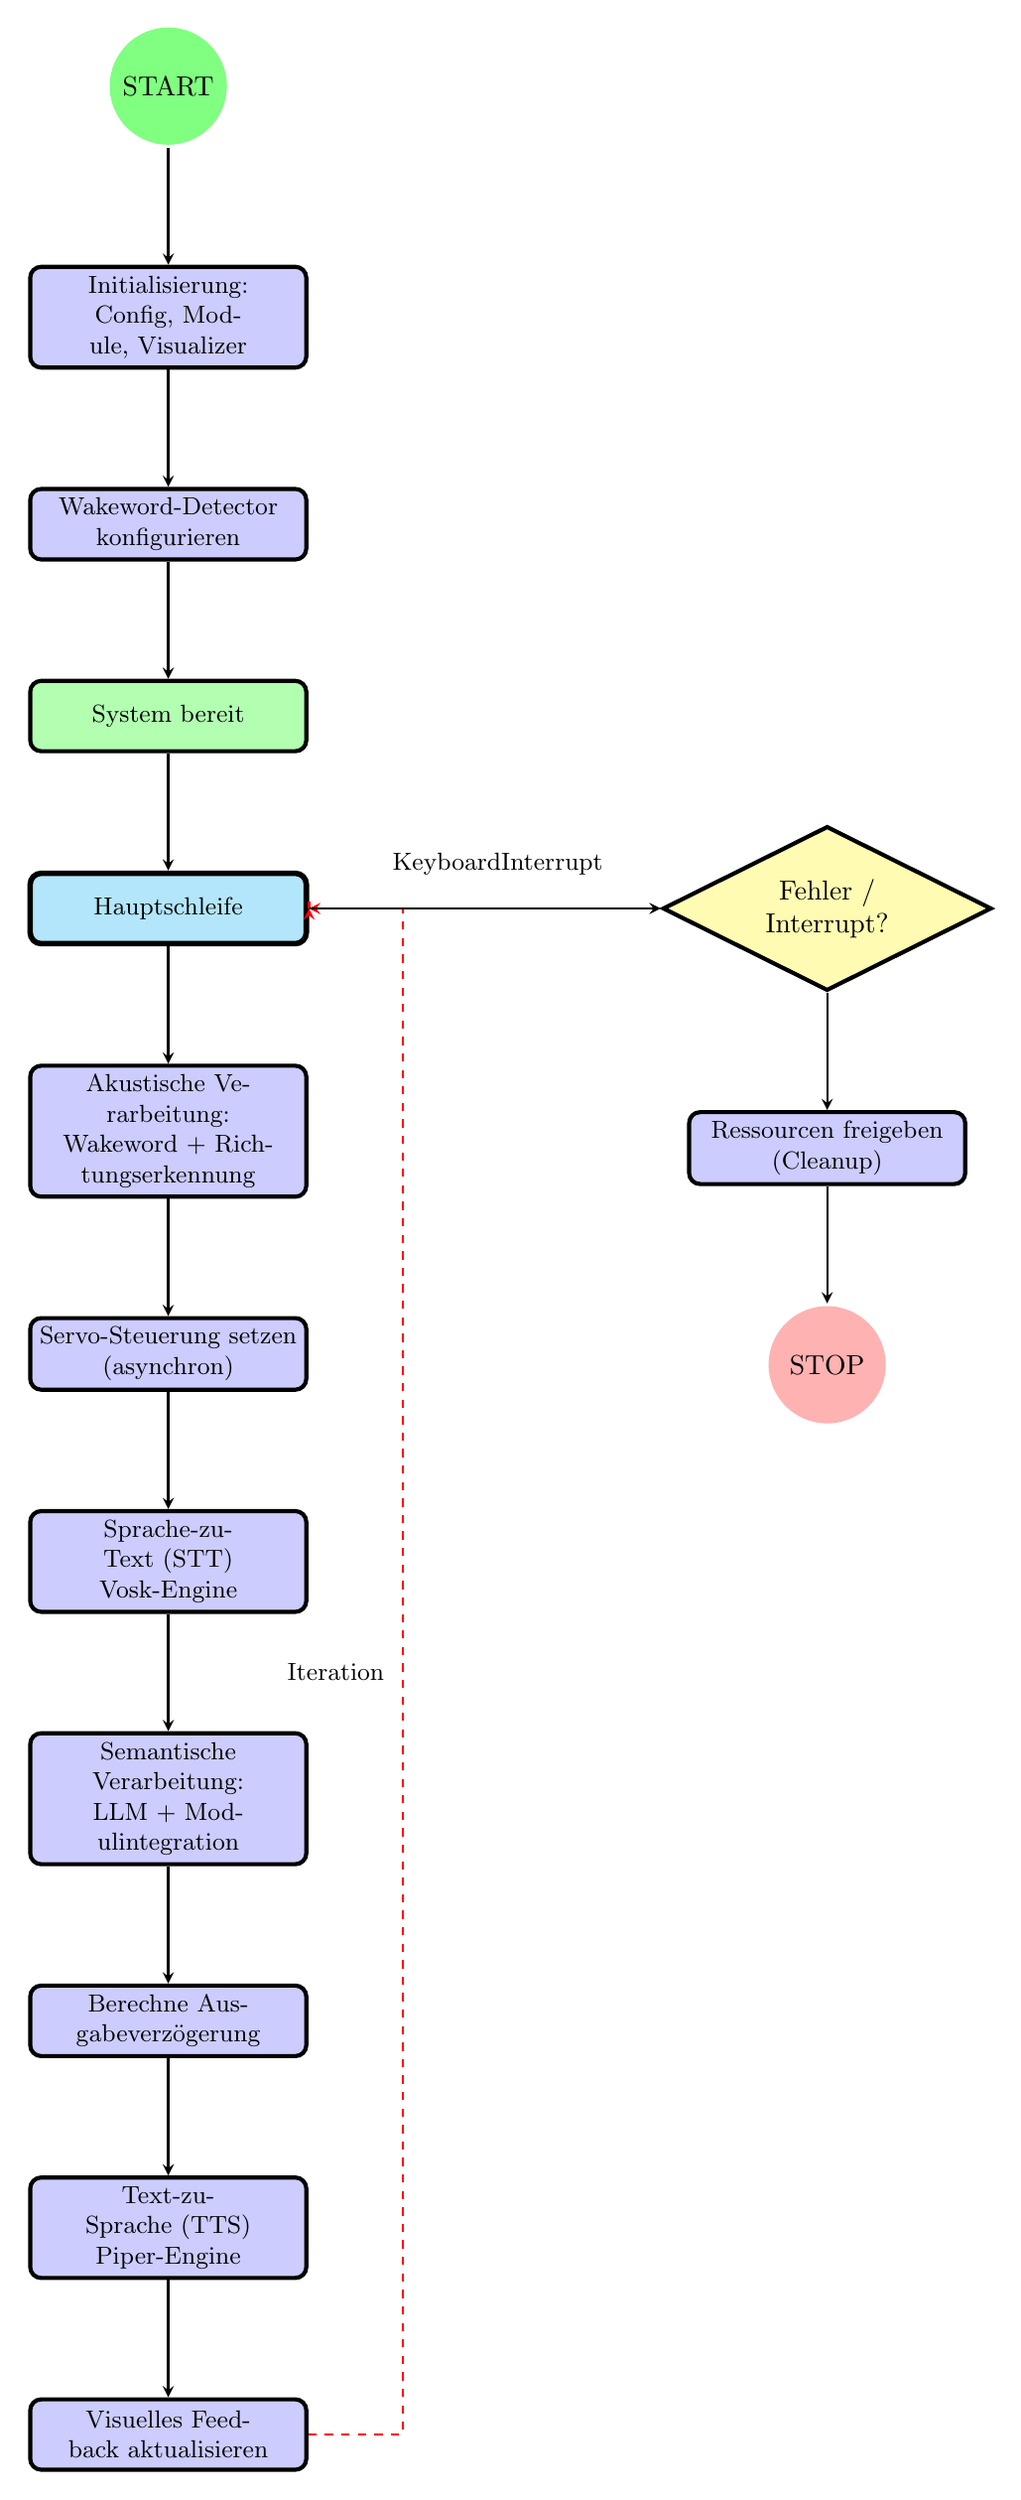
\begin{tikzpicture}[node distance=1.5cm]

% INITIALISIERUNGSPHASE
\node (start) [start] {START};
\node (init) [process, below=of start] {Initialisierung:\\Config, Module, Visualizer};
\node (detector) [process, below=of init] {Wakeword-Detector\\konfigurieren};
\node (ready) [process, below=of detector, fill=green!30] {System bereit};

% HAUPTSCHLEIFE - Eintritt
\node (mainloop) [process, below=of ready, fill=cyan!30, line width=2pt] {Hauptschleife};

% SCHRITT 1: Akustische Eingabe
\node (acoustic) [process, below=of mainloop] {Akustische Verarbeitung:\\Wakeword + Richtungserkennung};
\node (servo) [process, below=of acoustic] {Servo-Steuerung setzen\\(asynchron)};

% SCHRITT 2: Spracherkennung
\node (stt) [process, below=of servo] {Sprache-zu-Text (STT)\\Vosk-Engine};

% SCHRITT 3: LLM Verarbeitung
\node (llm) [process, below=of stt] {Semantische Verarbeitung:\\LLM + Modulintegration};

% SCHRITT 4: Sprachausgabe
\node (delay) [process, below=of llm] {Berechne Ausgabeverzögerung};
\node (tts) [process, below=of delay] {Text-zu-Sprache (TTS)\\Piper-Engine};

% Schleife zurück
\node (loop_back) [process, below=of tts] {Visuelles Feedback aktualisieren};

% Fehlerbehandlung/Cleanup
\node (error) [decision, right=4.5cm of mainloop] {Fehler /\\Interrupt?};
\node (shutdown) [process, below=of error] {Ressourcen freigeben\\(Cleanup)};
\node (exit) [end, below=of shutdown] {STOP};

% PFEILE - Initialisierung
\draw [arrow] (start) -- (init);
\draw [arrow] (init) -- (detector);
\draw [arrow] (detector) -- (ready);
\draw [arrow] (ready) -- (mainloop);

% PFEILE - Hauptschleife
\draw [arrow] (mainloop) -- (acoustic);
\draw [arrow] (acoustic) -- (servo);
\draw [arrow] (servo) -- (stt);
\draw [arrow] (stt) -- (llm);
\draw [arrow] (llm) -- (delay);
\draw [arrow] (delay) -- (tts);
\draw [arrow] (tts) -- (loop_back);

% PFEILE - Schleife zurück (rechts herum)
\draw [loop] (loop_back) -- +(3,0) |- ($(mainloop.east)+(0,0)$);
\draw [loop] ($(mainloop.east)+(0,0)$) -- (mainloop.east);

% PFEILE - Fehler/Cleanup
\draw [arrow] (mainloop.east) -- (error);
\draw [arrow] (error) -- (shutdown);
\draw [arrow] (shutdown) -- (exit);

% Beschriftung
\node at ($(mainloop)!0.5!(error)$) [above=0.3cm, font=\small] {KeyboardInterrupt};
\node at ($(loop_back)!0.5!($(mainloop.east)+(0,0)$)$) [right=0.5cm, font=\small] {Iteration};

\end{tikzpicture}

\end{document}
